
\par\vspace{5mm}
{\large \textbf{Pagination}}
\par\vspace{3mm}
In this section, users can view the results in a paginated format. The pagination control allows users to select the number of rows they want to display per page. Options such as **20**, **50**, **100**, and **200** rows can be selected, providing flexibility in viewing the data.

On the right side, there are navigation arrows that allow the user to move between pages. The **Previous** and **Next** buttons help users navigate through the results, while the current page number is displayed for clarity. This allows for easy browsing of large datasets without overwhelming the user with too much information at once.

\begin{figure}[ht]
  \centering  \colorbox{gray!20}{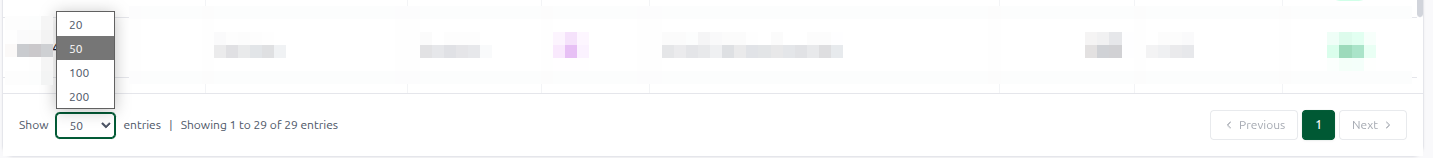
\includegraphics[width=.97\textwidth]{img/common/commonarea/results/R3Pageination.png}}  % Replace with the path to your image file

  \caption{Example of Pagination Control}
\end{figure}